\def \sst {\draw[cyan] (-2, -.9) -- (-.5, -.5);}
\def \tst {\draw[orange] (2, -.9) -- (.5, -.5);}

\def \os {\draw[blue, loosely dotted] (-2, 2) -- (-2, .5);}
\def \cupst {\draw[loosely dashed] (-.5, 2) -- (-.5, .5);}
\def \capst {\draw[red, loosely dashed] (.5, 2) -- (.5, .5);}
\def \ot {\draw[orange, loosely dash dot] (2, 2) -- (2, .5);}

\begin{subfigure}{.48\linewidth}
\caption{\label{}}
\centering
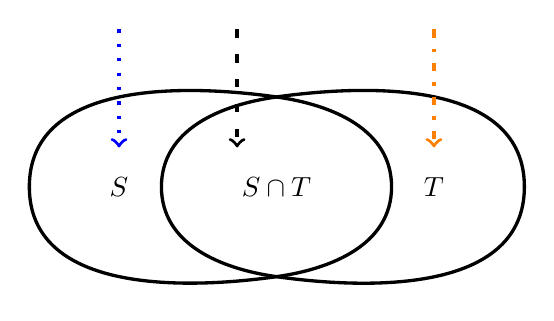
\begin{tikzpicture}[very thick]

\begin{scope}[every node/.style={inner sep=1cm}]
\node(s) at(-2,0) {$S$};
\node(st) at(0,0) {$S \cap T$};
\node(t) at(2,0) {$T$};
\end{scope}

\draw 
(s.west) to[out=90, in=172] 
(st.north) to[out=-8, in=90] 
(st.east) to[out=270, in=8]
(st.south) to[out=188, in=270]
(s.west)
;

\draw 
(t.east) to[out=90, in=8] 
(st.north) to[out=188, in=90] 
(st.west) to[out=270, in=172]
(st.south) to[out=-8, in=270]
(t.east)
;

\begin{scope}[->]
\os
\cupst
\ot
\end{scope}

\end{tikzpicture}
\end{subfigure}
%
\hfill
%
\begin{subfigure}{.48\linewidth}
\caption{\label{}}
\centering
\begin{tikzpicture}[very thick]

\begin{scope}[every node/.style={inner sep=1cm}]
\node(s) at(-2,0) {$S$};
\node(st) at(0,0) {$S \cap T$};
\node(t) at(2,0) {$T$};
\end{scope}

\draw[outline] 
(st.south) to[out=188, in=270]
(s.west) to[out=90, in=172] 
(st.north)
;
\draw 
(st.north) to[out=-8, in=90] 
(st.east) to[out=270, in=8]
(st.south)
;

\draw[outline] 
(st.south) to[out=-8, in=270]
(t.east) to[out=90, in=8] 
(st.north)
;
\draw 
(st.north) to[out=188, in=90] 
(st.west) to[out=270, in=172]
(st.south)
;

\begin{scope}[->]
\sst
\capst
\tst
\end{scope}

\end{tikzpicture}
\end{subfigure}


\begin{subfigure}{.48\linewidth}
\caption{\label{}}
\centering
\begin{tikzpicture}[very thick]

\begin{scope}[every node/.style={inner sep=1cm}]
\node(s) at(-2,0) {$S$};
\node(st) at(0,0) {$S \cap T$};
\node(t) at(2,0) {$T$};
\end{scope}

\draw 
(s.west) to[out=90, in=172] 
(st.north) to[out=-8, in=90] 
(st.east) to[out=270, in=8]
(st.south) to[out=188, in=270]
(s.west)
;

\draw[outline] 
(st.south) to[out=-8, in=270]
(t.east) to[out=90, in=8] 
(st.north) 
;
\draw 
(st.north) to[out=188, in=90] 
(st.west) to[out=270, in=172]
(st.south)
;

\begin{scope}[->]
\os
\cupst
\tst
\end{scope}

\end{tikzpicture}
\end{subfigure}
%
\hfill
%
\begin{subfigure}{.48\linewidth}
\caption{\label{}}
\centering
\begin{tikzpicture}[very thick]

\begin{scope}[every node/.style={inner sep=1cm}]
\node(s) at(-2,0) {$S$};
\node(st) at(0,0) {$S \cap T$};
\node(t) at(2,0) {$T$};
\end{scope}

\draw[outline] 
(st.south) to[out=188, in=270]
(s.west) to[out=90, in=172] 
(st.north)
;
\draw 
(st.north) to[out=-8, in=90] 
(st.east) to[out=270, in=8]
(st.south)
;

\draw 
(t.east) to[out=90, in=8] 
(st.north) to[out=188, in=90] 
(st.west) to[out=270, in=172]
(st.south) to[out=-8, in=270]
(t.east)
;

\begin{scope}[->]
\sst
\capst
\cupst
\ot
\end{scope}

\end{tikzpicture}
\end{subfigure}